\documentclass[10pt,twocolumn,letterpaper]{article}

\usepackage[pdf]{pstricks}
\usepackage{cvpr}
\usepackage{times}
\usepackage{epsfig}
\usepackage{graphicx}
\usepackage{amsmath}
\usepackage{amssymb,amsfonts}
\usepackage{bm}
\usepackage{xcolor}

% Include other packages here, before hyperref.

\usepackage{algorithm}
\usepackage{algorithmic}

%--------------------------------- Variable representation --------------------------------------------%
\DeclareMathOperator*{\E}{\mathbb{E}}
\providecommand{\trace}[1]{\ensuremath{tr}\{#1\}}% expectation operator
\providecommand{\cov}[2]{{\ensuremath{cov}}\{#1,#2\}}% covariance operator, \cov{x} {y}
\providecommand{\var}[1]{{\ensuremath{var}}\{#1\}}% variance operator
\providecommand{\re}[1]{{\ensuremath{Re}}\{#1\}}% real part
\providecommand{\ve}[1]{{\bm{#1}}} %
\providecommand{\mat}[1]{{\bm{#1}}} %
\providecommand{\est}[1]{{\widetilde {#1}}}
\DeclareMathOperator{\Real}{\mathbb{R}}
\DeclareMathOperator{\Complex}{\mathbb{C}}

\newcommand{\stateb}{\STATE \textbullet~}

% If you comment hyperref and then uncomment it, you should delete
% egpaper.aux before re-running latex.  (Or just hit 'q' on the first latex
% run, let it finish, and you should be clear).
\usepackage[pagebackref=true,breaklinks=true,letterpaper=true,colorlinks,bookmarks=false]{hyperref}

% \cvprfinalcopy % *** Uncomment this line for the final submission

\def\cvprPaperID{***} % *** Enter the CVPR Paper ID here
\def\httilde{\mbox{\tt\raisebox{-.5ex}{\symbol{126}}}}

% Pages are numbered in submission mode, and unnumbered in camera-ready
\ifcvprfinal\pagestyle{empty}\fi
\begin{document}

%%%%%%%%% TITLE
\title{Weakly supervised super resolution for plant and root imaging}

\author{Jose F. Ruiz-Munoz, Alina Zare \\
University of Florida, Department of Electrical and Computer Engineering, Gainesville, FL, USA\\
{\tt\small jruizmunoz@ufl.edu, azare@ece.ufl.edu}
\and
Jyothir K. Nimmagadda, Shuang Cui, James Baciak \\
University of Florida, Department of Material Sciences and Engineering, Gainesville, FL, USA\\
{\tt\small jyothir@ufl.edu, cuishuang413@ufl.edu, jebaciak@mse.ufl.edu}
% For a paper whose authors are all at the same institution,
% omit the following lines up until the closing ``}''.
% Additional authors and addresses can be added with ``\and'',
% just like the second author.
% To save space, use either the email address or home page, not both
% \and
% Second Author\\
% Institution2\\
% First line of institution2 address\\
%{\tt\small secondauthor@i2.org}
}

\maketitle
%\thispagestyle{empty}

%%%%%%%%% ABSTRACT
\begin{abstract}
    In this study, we propose a super-resolution (SR) algorithm that transforms low-resolution (LR) images into higher-quality images based on a generative adversarial network (GAN). The proposed approach aims to estimate super-resolved imagery that enhances the features which result in improved classification accuracy for analysis tasks of interest. This framework is suitable to improve the capability of a novel X-ray backscatter system (and similar tasks) where LR-HR pairs are not available for training. Our results show that the proposed approach allows creating super-resolved images appropriate for leaf-disease classification and X-ray back-scatter imaging of plant roots.
\end{abstract}

%%%%%%%%% BODY TEXT
\section{Introduction}
High-throughput image-based phenotyping facilitates the measurement of features of plants that are required for applications and studies such as crop production analysis, and the design of ecological models. This technology consists of tools of hardware and software that allows the acquisition and processing of the target biophysical data. Tasks that traditionally are carried out by visual inspection can be made efficiently by using a variety of imaging sensors~\cite{Fahlgren2015}. However, these sensors usually have resolution limitations or are not appropriate to acquire a certain type of data, e.g., below-ground biomass. In this paper, we develop a super-resolution (SR) algorithm to train a model that transforms low-resolution (LR) images into SR images. To this end, we require image level labels of LR images and high-resolution (HR) images without labels.

Digital signal processing (DSP) and machine learning (ML) techniques have been applied in phenotyping tasks such as detection, classification, and prediction~\cite{Singh2018}. Particularly, deep-learning has become very popular in the ML community but has not been extensively studied for plant phenotyping applications~\cite{Ubbens2017}. Nevertheless, it has a wide range of potential applications, e.g., in \cite{Ramcharan2017}, a method for disease detection based on a deep learning model is proposed, which is implemented in mobile devices for field-data analysis, and in \cite{Giuffrida2017}, a generative adversarial network (GAN) is used for data augmentation of plant images.

Image acquisition and processing on uncontrolled conditions is challenging in plant phenotyping since it implies handling issues such as uneven illumination, complex background or LR sensors. These complications result more noticeable for specific applications. In this study, we are particularly interested in the imaging of roots in situ, where it is difficult to distinguish the target from their surroundings~\cite{Tabb2018}. More advanced non-invasive techniques for this application include electrical capacitance and ground-penetrating radar. However, these sensors still have restrictions in depth and resolution~\cite{Araus2014}. As an alternative, X-ray backscatter radiography technology is being currently explored. In the first laboratory experiments, it has been possible to scan woody plant roots, root trees, and root vegetables buried up to 3 inches depth. An effective SR algorithm that complements the image formation process would allow the deployment of this technology to the field and its application on a variety of soil and species.

The SR problem consists of recovering HR images from LR images. Many SR approaches can be found in the DSP and ML literature. Applications such as medical diagnostic heavily rely on high-quality images~\cite{Zhang2012}. This is an inherently ill-posed problem, i.e., no unique solution exists~\cite{Hui2018}. Therefore, the SR methods require regularization terms to constrain the search space. 
Recently, GANs have been used to learn a transformation between two domains~\cite{Hong2018}. In the case of an SR application, a GAN is trained to map the LR domain into the HR domain~\cite{Ledig2017}. An SR method for plant images (trained with HR-LR pairs of images) is proposed in \cite{Yamamoto2017}. Their results show that this technique allows the improvement of the classification performance obtained by LR images.

SR algorithms promote the development of new alternatives to sense data, such as X-ray based sensors, since efficient algorithms can help to overcome weakness in hardware. The loss function of an SR problem is usually the mean squared error (MSE) between the estimated SR image and the original HR image plus the regularization term. An issue in SR methods is that MSE minimization does not avoid visual artifacts. Besides, some SR methods require training pairs of LR-HR examples~\cite{Zeyde2012}, which is a practical disadvantage.

In this paper, we proposed a weakly supervised GAN for increasing the resolution of LR plant and root images. This is a weakly supervised-approach since it uses image-level labels to learn to enhance lower level details. In this configuration, the regularization of the SR problem force the generated images to be both, ``realistic-like'' images and appropriate for classification. The remainder of this paper is divided as follows: Sec.~\ref{sec:methods} described the proposed method, Sec.~\ref{sec:experiments} includes details of the implementation of the experiments and the results on three types of data, and Sec.~\ref{sec:conclusion} concludes the study.

%-------------------------------------------------------------------------

\section{Methods}
\label{sec:methods}

\subsection{Adversarial Networks}

A basic generative adversarial network (GAN) consists of two nets ---a generator $G,$ and a discriminator $D$. On the adversarial configuration, these two nets play contrary roles, i.e., on the one hand, $G$ aims at generating ``realistic-like fake data'' capable of fooling $D$, whereas $D$ is continuously trained to classify fake data from real data~\cite{Goodfellow2014}. This formulation is expressed as follows
\begin{eqnarray}
\label{eq:gan}
\begin{aligned}
& \min_G \max_D \E_{\ve{x} \sim p(\ve{x})}[\log D(\ve{x})]\\
& +\E_{\ve{z} \sim p(\ve{z})}[\log (1 - D(G(\ve{z})))]  
\end{aligned}
\end{eqnarray}
where $\ve{x}$ denotes a real sample, and $\ve{z}$ is the input of the generator, that depending on the problem might be random noise, a lower-resolution sample, or a version of a sample in other domain.

\subsection{Classification loss function}

The parameters of a two-class classifier $C$ at the image level can be found solving
\begin{eqnarray}
\label{eq:cnet}
\min_C \E_{\ve{x} \sim p(\ve{x|L_0})}[\log C(\ve{x})] +  \E_{\ve{x} \sim p(\ve{x|L_1})}[1-\log C(\ve{x})]
\end{eqnarray}
where $C$ outputs the probability that its input $x$ comes from the target class distribution $p(x|L_1)$ and not from the non-target class distribution $p(x|L_0),$ i.e., if $C(x)=1$ the classifier ensures that $x$ is a sample of the target class $L_1,$ on the other hand, $C(x)=0$ indicates that $x$ is a sample of the non-target class $L_0$.

\subsection{Weakly supervised adversarial network}

Our proposed method is illustrated in Fig.~\ref{fig:cgan}. The network is divided into three stages, i) $G$ that generates SR images from LR inputs, ii) $D$ that classifies HR images from SR images, and iii) $C$ that is our additional regularization to the traditional GAN, which allows enhancing relevant aspects in the generated images for classification purposes. Figure~\ref{fig:D_net} shows the architecture for $C$ and $D.$ We use the same architecture for both of them. Likewise, Fig.~\ref{fig:G_net} shows the generator architecture.

\begin{figure}[h]
\begin{center}
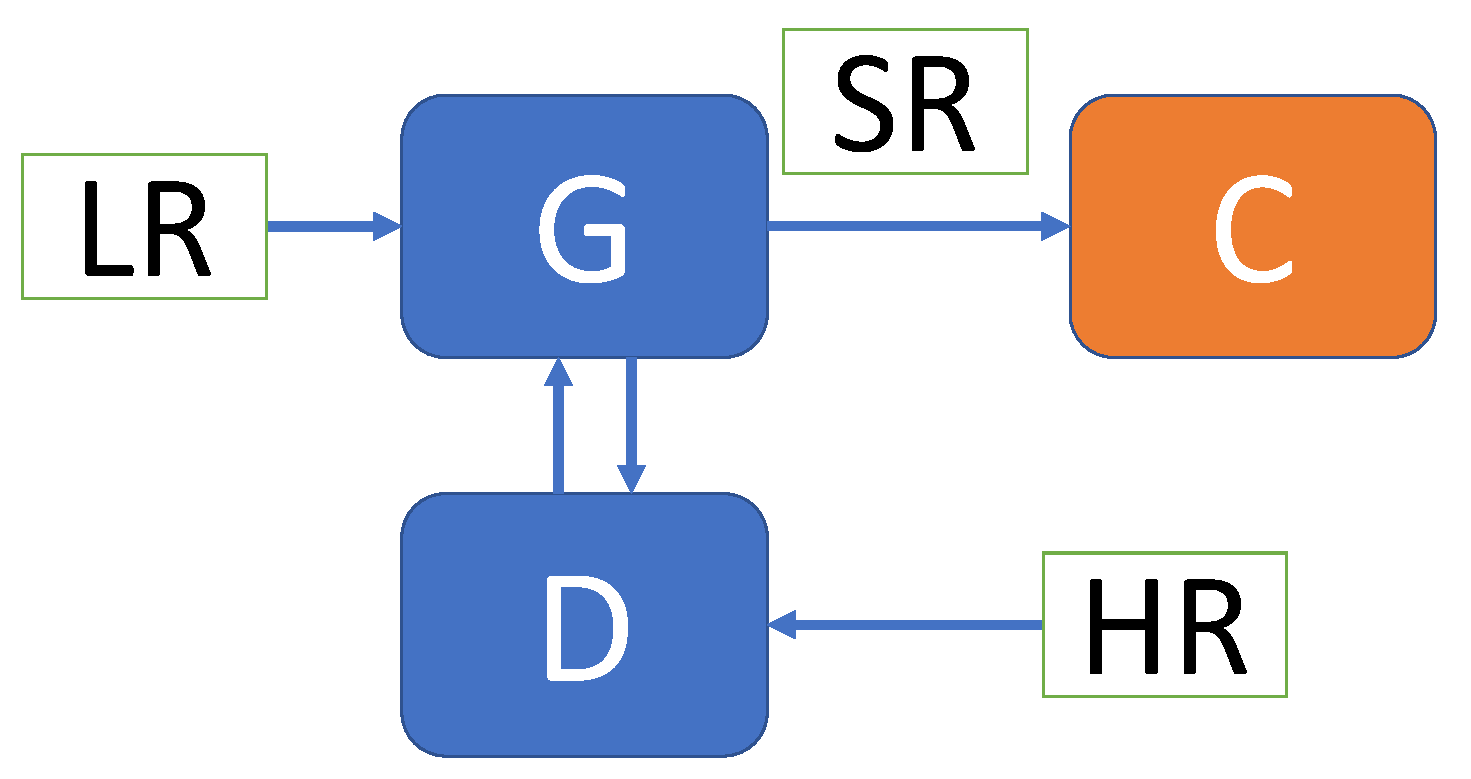
\includegraphics[scale=0.25]{cgan.pdf}
\end{center}
   \caption{Generation of SR images by an adversarial network. This method consists of three blocks: generator ($G$), discriminator ($D$), and classifier ($C$).}
\label{fig:cgan}
\end{figure}

\begin{figure}[h]
\begin{center}
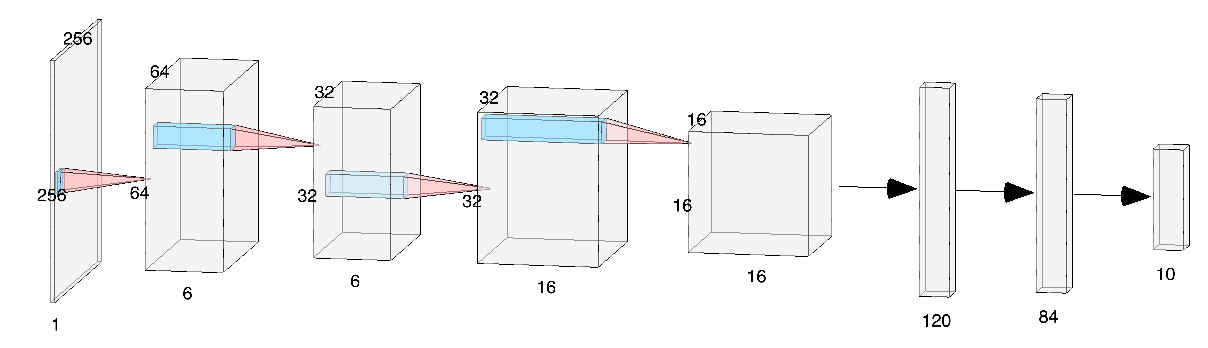
\includegraphics[scale=0.20]{D_net.png}
\end{center}
   \caption{Discriminator ($D$) and classifier ($C$) network. Same architecture is used for each one of them.}
\label{fig:D_net}
\end{figure}

\begin{figure}[h]
\begin{center}
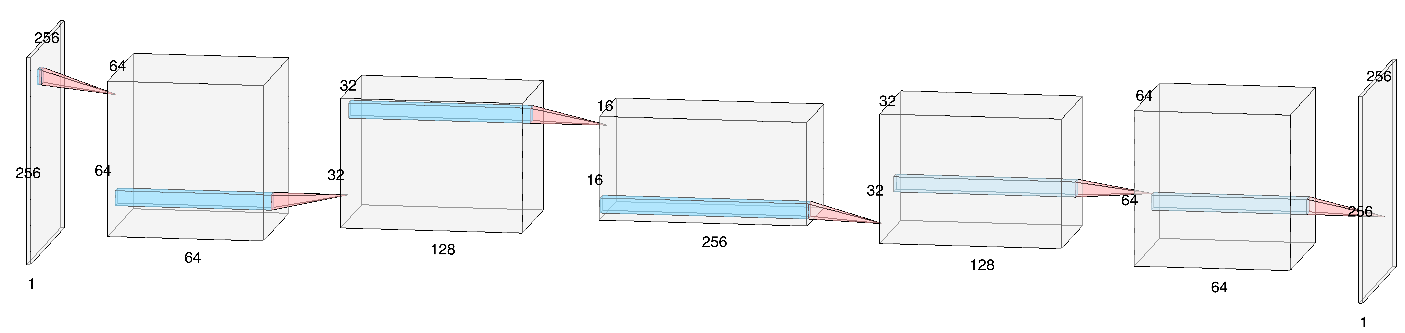
\includegraphics[scale=0.17]{G_net.png}
\end{center}
\label{fig:G_net}
\caption{Generator (G) network.}
\end{figure}

Our proposed formulation is expressed as follows
\begin{eqnarray}
\label{eq:srcgan}
\footnotesize
\begin{aligned}
& \min_{C,G} \max_D \E_{\ve{z} \sim p(\ve{z|L_0})}[\log C(G(\ve{z}))] \\ & +  \E_{\ve{z} \sim p(\ve{z|L_1})}[1-\log C(G(\ve{z}))] \\ & + \E_{\ve{x} \sim p(\ve{x})}[\log D(\ve{x})] + \E_{\ve{z} \sim p(\ve{z})}[\log (1 - D(G(\ve{z})))].
\end{aligned}
\end{eqnarray}


Note that $G$ maps the labeled-LR data $z$ to a higher-resolution domain. Since we assume that the HR labels are unknown, the classifier is trained with the SR data. Algorithm~\ref{alg:srcgan} contains the pseudo-code.

\begin{algorithm}[h!]
    \caption{Minibatch gradient descent training of the \textbf{weakly supervised adversarial network}.}
    \label{alg:srcgan}
    \begin{algorithmic}
    \FOR{number of training iterations}
    \stateb Sample minibatch of $m$ samples $\{x_1,\ldots, x_m\}$ from HR data distribution $p(x)$.
    \stateb Sample minibatch of $m$ samples $\{y_1,\ldots, y_m\}$ from LR data distribution $p(y|L_0)$.
    \stateb Sample minibatch of $m$ samples $\{z_1,\ldots, z_m\}$ from LR data distribution $p(z|L_1)$.
    \stateb Update the classifier by descending its stochastic gradient
    \[\nabla_{\theta_c} \frac{1}{m} \sum_{i=1}^m \left[\log C(G(y_i)) + \log(1 - C(G(z_i))) \right]. \]
    \stateb Update the discriminator by descending its stochastic gradient
    \[
    \begin{aligned}
    \nabla_{\theta_d} \frac{1}{m} \sum_{i=1}^m \left[\log D(z_i) + \log(1- D(G(x_i))) \right. \\ \left. + \log(1- D(G(y_i))) \right].
    \end{aligned}
    \]
    \stateb Update the generator by descending its stochastic gradient
    \[
    \begin{aligned}
    \nabla_{\theta_{g}} \frac{1}{m} \sum_{i=1}^m \left[\log C(G(y_i)) + \log(1 - C(G(z_i))) \right. \\ \left. + \log(1- D(G(x_i)))+\log(1- D(G(y_i))) \right].
    \end{aligned}
    \]
\stateb Update the decoder by descending its stochastic gradient
    \ENDFOR
    \STATE The gradient-based updates can use any standard gradient-based learning rule.
    \end{algorithmic}
\end{algorithm}

%------------------------------------------------------------------------
\section{Experiments}
\label{sec:experiments}

We perform experiments on two datasets. The first one contains 3719 images (from PlantVillage project~\cite{Hughes2015}) of tomato leaves divided into two classes: Healthy (training: 1392; test: 200) and Bacteria (training: 1927; test: 200). The second dataset consists of 8 buried-roots scans, 4 soil scans, and 3 scans of root vegetables, which were acquired by the authors using a novel X-ray backscatter system. As gradient-based learning rule, we use the Adaptive Moment Estimation (Adam).

\subsection{Disease Classification}

We apply our method to an image-based plant disease classification task~\cite{Mohanty2016}. We consider the original grayscale images ($256\times 256$) of the PlantVillage dataset as HR data. We create the LR versions of this images by downscaling 2 (LR2x: $128\times 128$), 4 (LR4x: $64\times 64$), 8 (LR8x: $32\times 32$), or 16 (LR16x: $16\times 16$) times and upscaling them again to $256\times 256$ by a bicubic interpolation.

Table~\ref{tab:results} shows the classification accuracy in a test set (200 images per class) at different resolutions when training two classifiers: i) the baseline classifier (network without the GAN) that is trained with 100 epochs of HR and LR images (each time that an image is selected is randomly downscaled, with the same probability, at LR2x, LR4x, LR8x, LR16x, or the original resolution is maintained), and ii) the SR-classifier (network that includes the proposed method: classifier together with the GAN that generates SR images). These results show that the SR-classifier outperforms the baseline classifier at every single resolution tested. Furthermore, the SR-classifier performs better when classifying the original images. We attribute this result to the fact that a more homogeneous distribution provided by the GAN might facilitate the classifier training, in contrast to the heterogeneous distribution that the classifier observes when trained directly with HR and LR data. Additionally, we observe that the baseline classifier accuracy decreases at LR scales, whereas the SR-accuracy is affected only at the two lowest scales (8x and 16x). Figure~\ref{fig:srimages} contains some examples of HR, LR, and SR of each class (Tomato - healthy and Tomato - bacterial spot).

\begin{table}[h]
\caption{Classification performance on the PlantVillage dataset applied to a test set.}
\label{tab:results}
\centering
\begin{tabular}{|c|c|c|}
\hline
  Downscaling & Classifier & SR-Classifier \\
\hline
\hline
None & 83.7 & \textbf{88.3} \\
2x & 82.7 & \textbf{90.3} \\
4x & 81.3 & \textbf{89.7} \\
8x & 81.0 & \textbf{85.5} \\
16x & 71.7 & \textbf{83.5} \\
\hline
\end{tabular}
\end{table}

\begin{figure*}[h]
\begin{center}
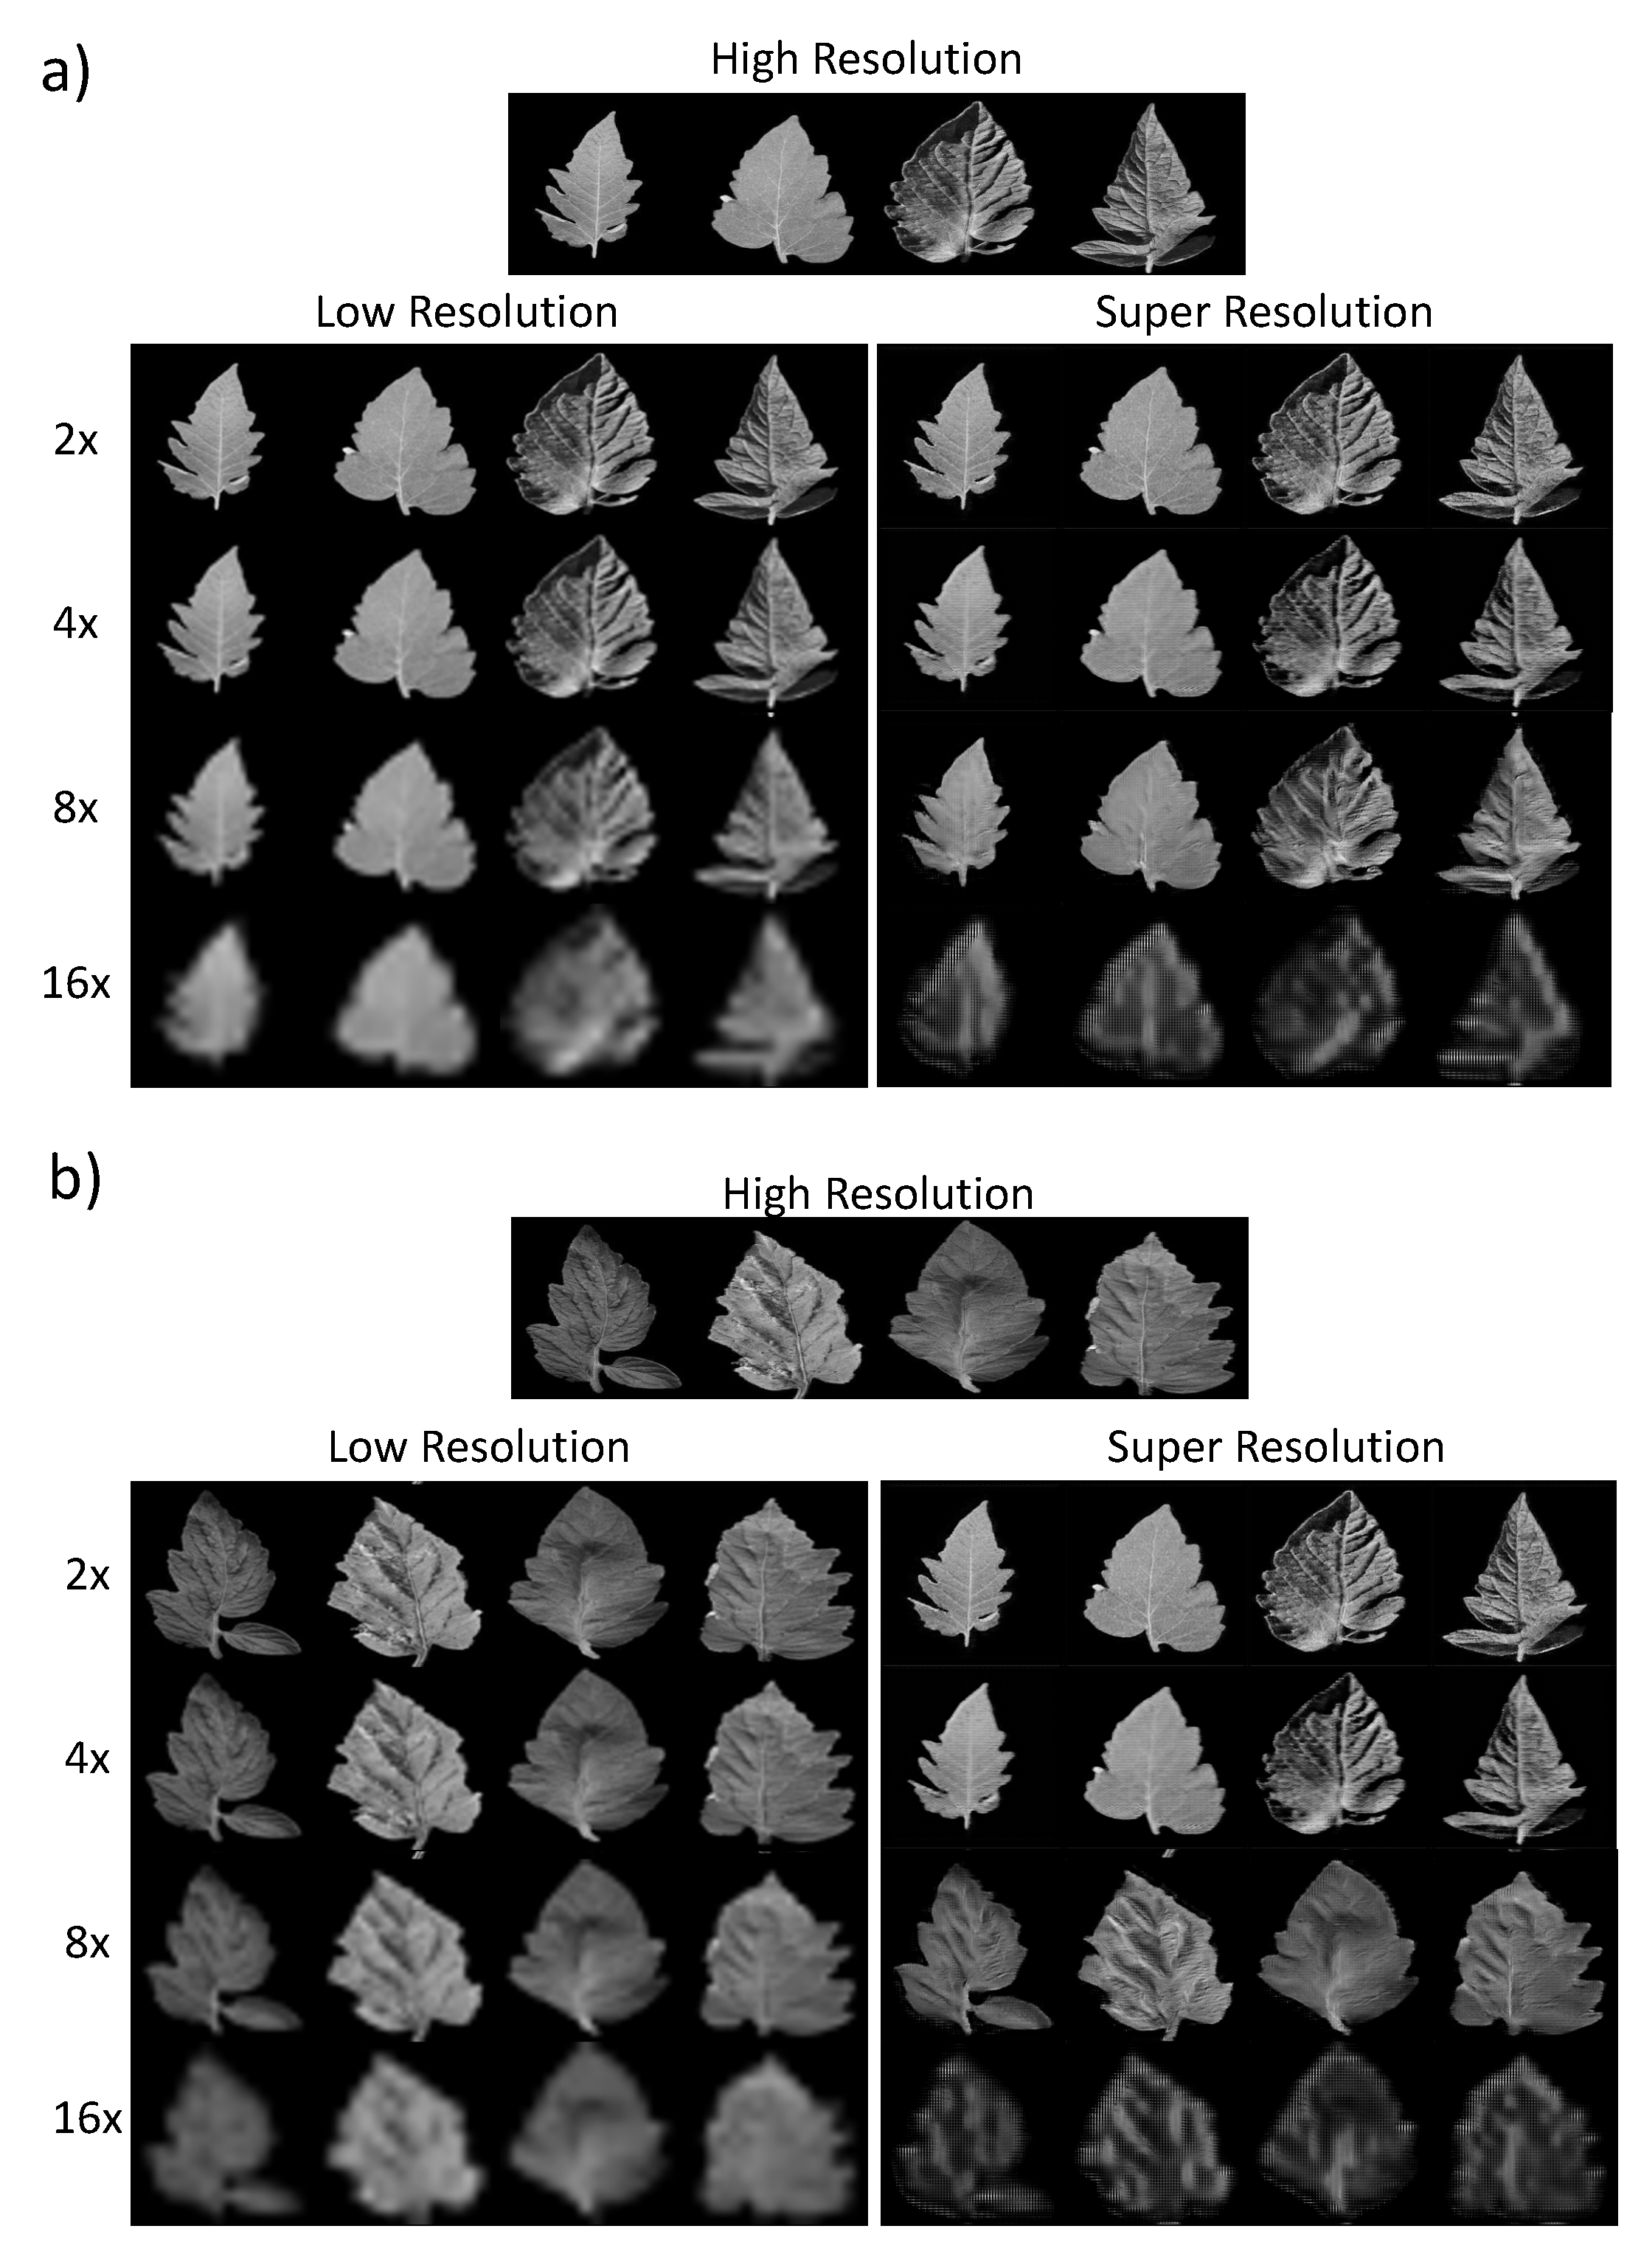
\includegraphics[scale=0.35]{results/srimages.pdf}
\end{center}
   \caption{a) Tomato - healthy. b) Tomato - bacterial spot} 
\label{fig:srimages}
\end{figure*}

\subsection{X-ray backscatter radiography data}

Aiming at scanning roots of plants in a non-invasive and non-destructive way, we developed a prototype device based on X-ray backscatter radiography technology~\cite{Kelley2019}. The X-ray backscatter imaging has the advantage of being single-sided imaging technique, which can be used for the non-destructive examination of buried roots. The X-ray backscatter prototype utilizes the fan beam geometry and the segmented linear detector arrays to collect the data~\cite{Cui2017}. A 2D motion table was used for scanning the target. This motion table was programmed to work with the data acquisition system to produce good quality X-ray backscatter images of roots and soil. For the class ``root,'' we scanned five pieces of plant and tree roots buried at 3 inches in potting soil, likewise, for the class ``soil,'' we scanned four images of only potting soil. As HR data, we manually edit one of the root images to enhance the root-soil contrast. Given the reduced amount of data to train the network, we create 100 images per class by randomly taking chunks of half of the size of the images and applying rotations. Figure~\ref{fig:srtest} shows SR applied to the X-ray backscatter radiography images. We test the method on images of potato, cassava, and radish buried at 3 inches (Fig.~\ref{fig:srtest} contains also the segmentation of these images, obtained by applying a threshold to the output of the first convolutional layer of the classifier). These results show that the SR method improves the contrast, but more training data is needed to enhance details of the roots.

\begin{figure*}[h]
\begin{center}
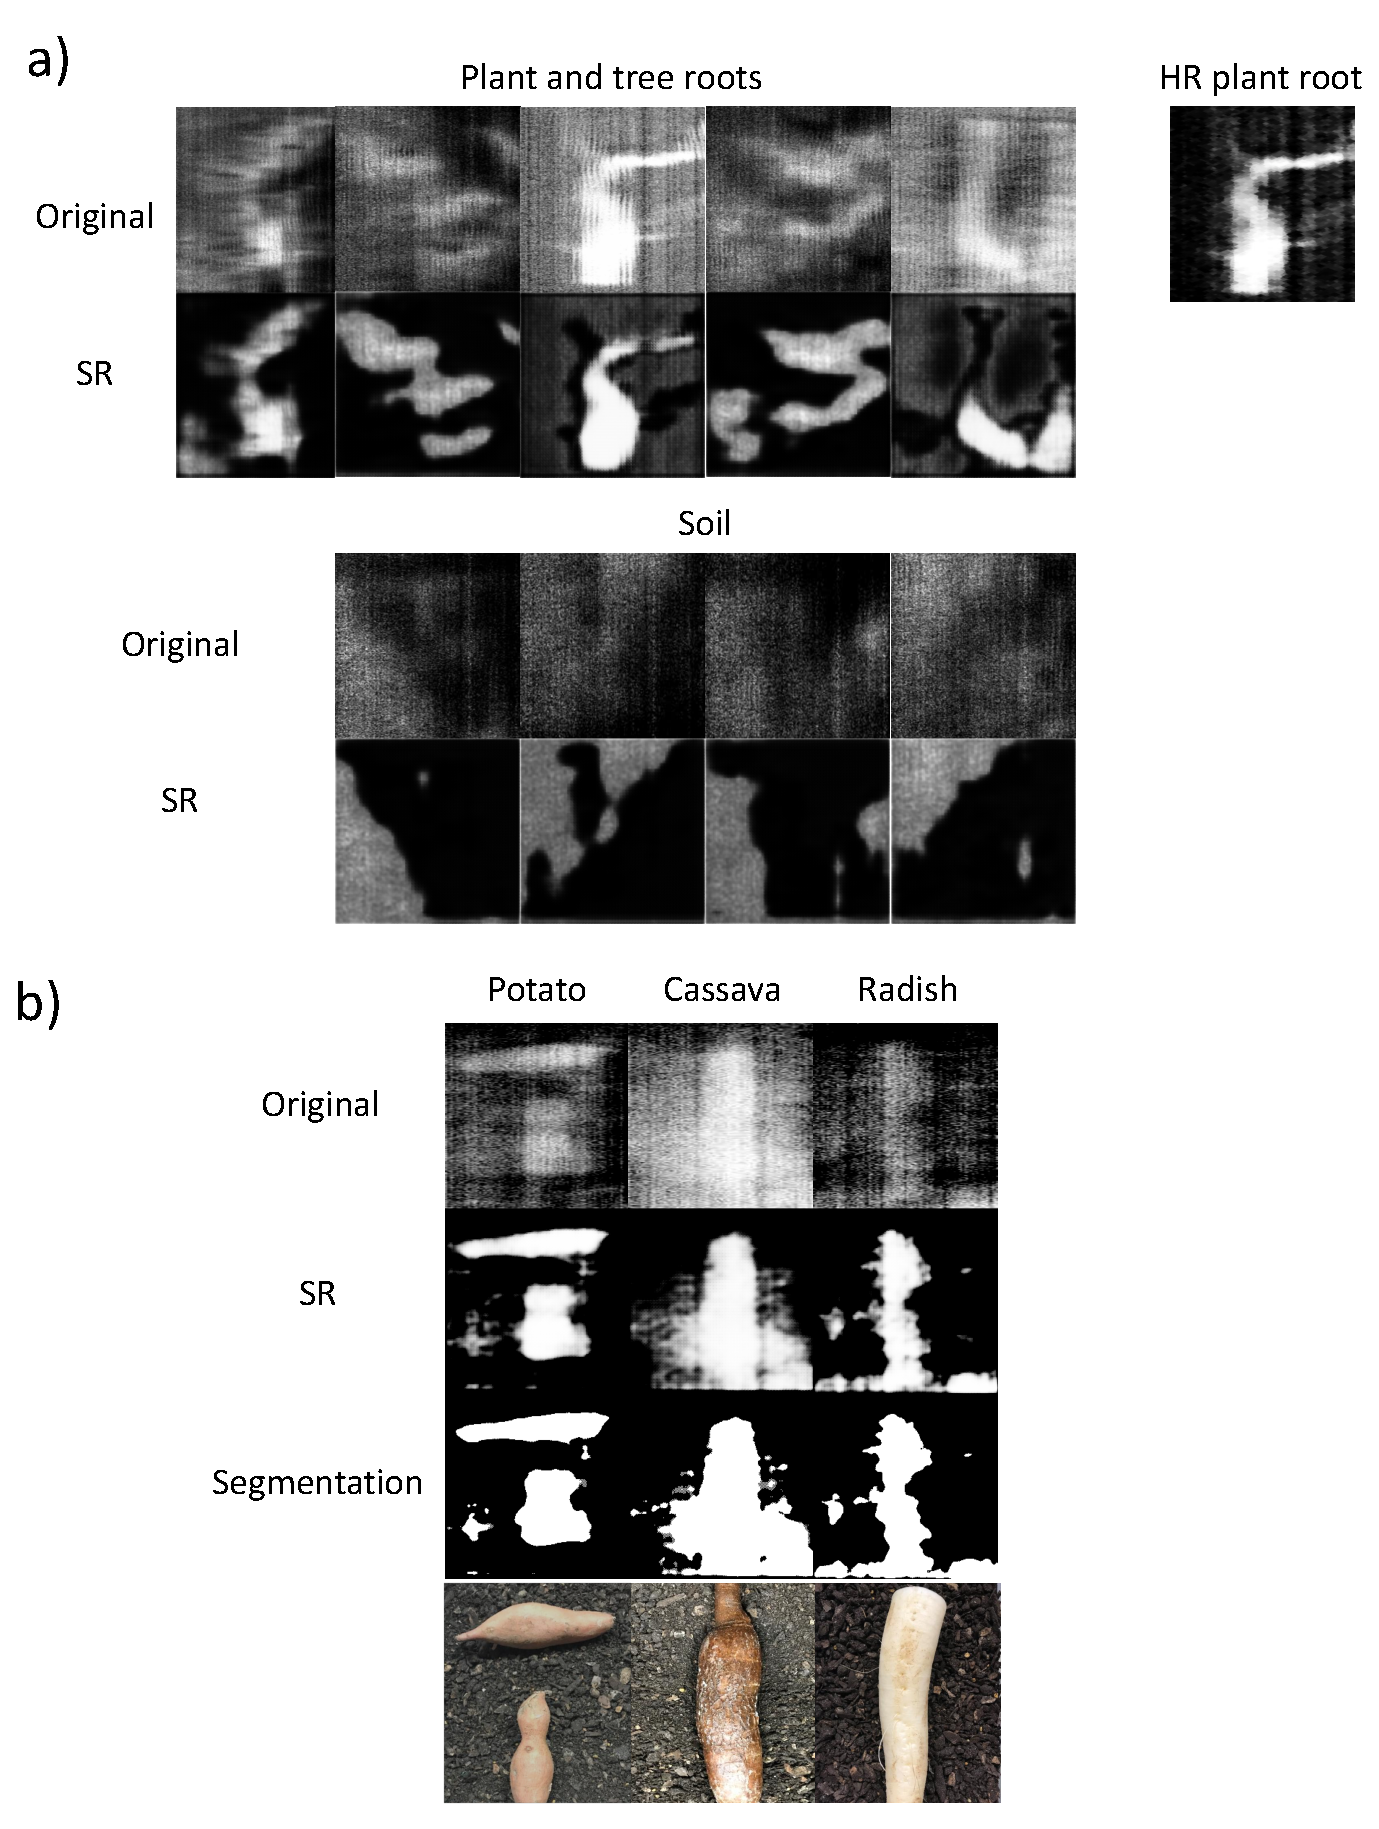
\includegraphics[scale=0.60]{results/srxray.pdf}
\end{center}
   \caption{SR applied to X-ray backscatter images. a) Training data; b) Test data}
\label{fig:srtest}
\end{figure*}

\section{Concluding remarks}
\label{sec:conclusion}

We proposed an SR method to create images that are both, similar to HR images and appropriate for a classification task. For this purpose, we use an adversarial configuration where a generator intends to fool a discriminator (trained to distinguish between HR and SR images) and, at the same time, to reduce the classification error. Results show that our method helps to improve the classification accuracy. Additionally, we use this method to enhance the contrast and facilitate the segmentation of noisy and LR images such as X-ray backscatter radiography images of buried roots. A practical advantage of our method is that it does not require pairs of LR-HR images for training.

As future work, we plan to acquire more X-ray backscatter radiography images of soil and roots, as well as apply the method to 3D data, e.g., CT scans. Also, this SR method might be considered as a preprocessing stage for applications such as feature extraction or segmentation. Finally, since the generator maps the original data into one distribution (in our experiments, the distribution of the HR data), this configuration might be applied in classification problems where the signals are acquired by different sensors.

%\clearpage

{\small
\bibliographystyle{ieee}
\bibliography{egbib}
}

\end{document}

